\documentclass[14pt]{extarticle}
\usepackage[utf8]{inputenc}
\usepackage[T1]{fontenc}
\usepackage[spanish,es-lcroman]{babel}
\usepackage{amsmath}
\usepackage{amsthm}
\usepackage{physics}
\usepackage{tikz}
\usepackage{float}
\usepackage{calc}
\usepackage[autostyle,spanish=mexican]{csquotes}
\usepackage[per-mode=symbol]{siunitx}
\usepackage{gensymb}
\usepackage{multicol}
\usepackage{enumitem}
\usepackage{setspace}
\usepackage[left=2.00cm, right=2.00cm, top=2.00cm, 
     bottom=2.00cm]{geometry}
\usepackage{Estilos/ColoresLatex}
\usepackage{makecell}
\usepackage{subcaption}

% \usepackage[sfdefault]{roboto}  %% Option 'sfdefault' only if the base font of the document is to be sans serif
% \usepackage[T1]{fontenc}

\usepackage{scalerel}[2016-12-29]
\def\stretchint#1{\vcenter{\hbox{\stretchto[440]{\displaystyle\int}{#1}}}}
\def\scaleint#1{\vcenter{\hbox{\scaleto[3ex]{\displaystyle\int}{#1}}}}
\def\bs{\mkern-12mu}

\newcommand{\textocolor}[2]{\textbf{\textcolor{#1}{#2}}}
\sisetup{per-mode=symbol}
\decimalpoint
\sisetup{bracket-numbers = false}
\newlength{\depthofsumsign}
\setlength{\depthofsumsign}{\depthof{$\sum$}}
\newcommand{\nsum}[1][1.4]{% only for \displaystyle
    \mathop{%
        \raisebox
            {-#1\depthofsumsign+1\depthofsumsign}
            {\scalebox
                {#1}
                {$\displaystyle\sum$}%
            }
    }
}

\title{\vspace*{-2cm} Aberraciones}
\date{ }

\begin{document}
\maketitle

\section{Introducción.}

Hasta el tema anterior se han hecho muchas simplificaciones con el objeto de poder estudiar las características y propiedades más sobresalientes de los sistemas ópticos. Supusimos que todos los rayos que salen de un punto en el objeto llegan a un punto común en la imagen. Esto es sólo aproximadamente válido y una consecuencia de considerar sólo rayos paraxiales.

Entre las aproximaciones más importantes está el haber sustituido el seno del ángulo por el valor del ángulo en radianes. Esta aproximación es muy buena para aberturas y campos pequeños, pero es necesario tomar en cuenta más términos de la serie del seno cuando éstos crecen, haciendo más grandes los ángulos. La \textit{óptica geométrica que considera sólo rayos paraxiales recibe el nombre de óptica de primer orden o gaussiana}. Aunque esta óptica no es exacta, es muy útil, pues con ella se pueden calcular distancia focal, las posiciones de objeto e imagen, los planos principales, etcétera.

\subsection{Aberraciones de primer orden y alto orden.}

Si se remplazan los senos de los ángulos por los dos primeros términos de la serie se obtiene la llamada \textit{teoría de tercer orden}, con la que se pueden obtener efectos secundarios que no prevé la teoría de primer orden. Las teorías de alto orden incluyen además otros términos de la serie. A continuación se estudiarán los efectos ópticos, llamados \textbf{aberraciones}, que hacen que la calidad de las imágenes no sea tan buena como es deseable.

La teoría de primer orden predice que un sistema óptico formado por lentes tiene diferentes distancias focales para distintos colores. Estas variaciones están relacionadas con el cambio del índice de refracción con el color. Esta variación de la distancia focal hace que tanto la posición como el tamaño de la imagen sean diferentes para cada color. El cambio en la posición es lo que se conoce como \textit{aberración cromática axial} y el cambio de tamaño como \textit{aberración cromática lateral}. Estas aberraciones son las únicas que puede predecir la teoría de primer orden y aparecen cuando la luz que ilumina el objeto es blanca.

Aun si la luz es monocromática, aparecen aberraciones que no puede predecir la óptica de primer orden. Si el objeto es puntual, la imagen no necesariamente lo es, debido a la presencia de las aberraciones monocromáticas. Éstas se pueden calcular en forma aproximada con la teoría de tercer orden. Mayor exactitud sólo se puede lograr con aproximaciones de orden superior, considerando más términos en el desarrollo del seno. Otra alternativa para calcularla con más precisión es hacer el trazo trigonométrico exacto de los rayos a través del sistema.

Las aberraciones monocromáticas se pueden observar tanto cuando la luz que forma la imagen es blanca como cuando es monocromática. A estas aberraciones se les conoce también como \textit{aberraciones de Seidel} y son las cinco siguientes:
\begin{enumerate}[label=\roman*)]
\item Esfericidad.
\item Coma.
\item Astigmatismo.
\item Distorsión.
\item Curvatura de campo.
\end{enumerate}
En seguida se estudiarán con algún detalle cada una de estas aberraciones y la forma de evitarlas.

\section{Aberración cromática axial.}

Cuando las imágenes roja, amarilla y azul de un objeto que emite estos colores están en planos diferentes, se dice que la lente tiene \textit{aberración cromática longitudinal o axial}. Se podría lograr que las imágenes azul y roja coincidieran en un solo plano, combinando dos o más lentes que tuvieran aberraciones cromáticas opuestas. A tal sistema se le da el calificativo de \textit{acromático}.

El hecho de que las imágenes roja y azul estén en un solo plano no implica que la imagen amarilla también esté en el mismo plano. Si combinando tres o más lentes se hacen coincidir los tres colores, tenemos un sistema \textit{apocromático}.

El sistema es acromático si los focos rojo y azul coinciden, pero hay que notar que esto implica que las distancias focales son iguales sólo si además los planos principales rojo y azul coinciden.

\subsection{Cálculo de un doblete acromático.}

Una lente positiva siempre tendrá aberración cromática, pero ésta se puede eliminar si se ponen en contacto dos lentes, una positiva y una negativa, de diferente tipo de vidrio. En un sistema de dos lentes delgadas en contacto, los planos principales para diferentes colores coinciden, ya que la distancia focal efectiva es igual a la distancia focal posterior. Así, el sistema será acromático si la distancia focal para el rojo es igual a la distancia focal para el azul. Esta lente compuesta se muestra en la figura (\ref{fig:figura_V_01}):
\begin{figure}[H]
    \centering
    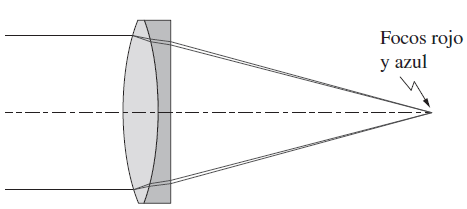
\includegraphics[scale=1]{Imagenes/Aberraciones_01.png}
    \caption{Corrección de la aberración cromática axial en un doblete.}
    \label{fig:figura_V_01}
\end{figure}
A continuación se calculará un doblete acromático, donde se usará el subíndice $1$ para las variables referentes a la primera lente y el subíndice $2$ para las variables referentes a la segunda lente. Se utilizarán los subíndices $C$ y $F$ para las variables relativas a los colores rojo y azul respectivamente.

Las distancias focales efectivas del doblete para los colores rojo (línea $C$) y azul (línea $F$) están dadas por la ecuación:
\begin{align}
\dfrac{1}{F_{C}} = \dfrac{1}{f_{1C}} + \dfrac{1}{f_{2C}}
\label{eq:ecuacion_V_01}
\end{align}
y
\begin{align}
\dfrac{1}{F_{F}} = \dfrac{1}{f_{1F}} + \dfrac{1}{f_{2F}}
\label{eq:ecuacion_V_02}
\end{align}
Para que el sistema sea acromática se requiere que $F_{C} = F_{F}$, es decir:
\begin{align}
\dfrac{1}{f_{1C}} - \dfrac{1}{f_{1F}} + \dfrac{1}{f_{2C}} - \dfrac{1}{f_{2F}} = 0
\label{eq:ecuacion_V_03}
\end{align}
Escribiendo la ecuación del fabricante de lentes:
\begin{align*}
\dfrac{1}{f} = (n - 1) \left( \dfrac{1}{r_{1}} - \dfrac{1}{r_{2}} \right)
\end{align*}
en la forma:
\begin{align}
\dfrac{1}{f} = (n - 1) \, K
\label{eq:ecuacion_V_04}
\end{align}
se puede escribir la ecuación (\ref{eq:ecuacion_V_03}) como:
\begin{align}
(n_{1C} - n_{1F}) \, K_{1} + (n_{2C} - n_{2F}) \, K_{2} = 0
\label{eq:ecuacion_V_05}
\end{align}
Definiendo la distancia focal de una lente como la distancia focal que tiene la lente para la luz amarilla, que es aproximadamente el centro del espectro visible, y representando el amarillo por el subíndice $D$, podemos escribir:
\begin{align}
\dfrac{1}{f_{1}} = \left( n_{1D} - 1 \right) \, K_{1}
\label{eq:ecuacion_V_06}
\end{align}
y
\begin{align}
\dfrac{1}{f_{21}} = \left( n_{2D} - 1 \right) \, K_{2}
\label{eq:ecuacion_V_07}
\end{align}
Conviene en la ecuación (\ref{eq:ecuacion_V_05}) poner $K_{1}$ y $K_{2}$ en función de las distancias focales $f_{1}$ y $f_{2}$ para el amarillo, por ser éstas las cantidades más fácilmente medibles. Así que:
\begin{align}
\dfrac{\left( n_{1c} - n_{1F} \right)}{f_{1} \left( n_{1D} - 1 \right)} + \dfrac{\left( n_{2c} - n_{2F} \right)}{f_{2} \left( n_{2D} - 1 \right)} = 0
\label{eq:ecuacion_V_08}
\end{align}
Recordemos ahora la definición dada en el capítulo I de un número que define la dispersión cromática del vidrio óptico, llamado \textit{constante de Abbe o número V}. Ésta es una constante que suministra el fabricante del vidrio óptico en la forma siguiente:
\begin{align}
V = \dfrac{n_{D} - 1}{n_{C} - n_{F}}
\label{eq:ecuacion_V_09}
\end{align}
Por lo tanto, de la ecuación (\ref{eq:ecuacion_V_08}), la condición de acromatismo es:
\begin{align}
f_{1} \, V_{1} = - f_{2} \, V_{2}
\label{eq:ecuacion_V10}
\end{align}
Se puede deducir entonces que las distancias focales de las componentes están dadas por:
\begin{align}
f_{1} = F \, \dfrac{V_{1} - V_{2}}{V_{1}}
\label{eq:ecuacion_V_11}
\end{align}
y
\begin{align}
f_{2} = F \, \dfrac{V_{2} - V_{1}}{V_{2}}
\label{eq:ecuacion_V_12}
\end{align}
Estas ecuaciones nos permiten calcular las distancias focales $f_{1}$ y $f_{2}$ de las componentes del doblete acromático.

Newton midió la dispersión, aunque no conocía el número de Abbe, de la mayoría de los vidrios conocidos en su tiempo. De sus resultados concluyó que era imposible hacer una lente acromática. Algunos años más tarde Fraunhofer encontró que Newton estaba equivocado, y construyó la primera lente acromática.
Si se grafica el índice de refracción contra el número de Abbe de los vidrios ahora conocidos, vemos que todos se encuentran dentro de una región relativamente pequeña.

\subsection{Cálculo de un doblete apocromático.}

Como ya se mencionó, el que los focos rojo y azul de un doblete coincidan no es condición suficiente para que el foco amarillo coincida con ellos. Un sistema donde los tres colores coinciden se dice que es \textit{apocromático}. No es difícil demostrar que un doblete es apocromático si además de satisfacer la ecuación (\ref{eq:ecuacion_V_08}) también satisface la siguiente:
\begin{align}
\dfrac{n_{F1} - n_{D1}}{n_{F1} - n_{C1}} = \dfrac{n_{F2} - n_{D2}}{n_{F2} - n_{C2}}
\label{eq:ecuacion_V_13}
\end{align}
La razón de dispersión parcial de un video se define como:
\begin{align}
P = \dfrac{n_{D} - n_{C}}{n_{F} - n_{C}} =  1 - \dfrac{n_{F} - n_{C}}{n_{F} - n_{C}}
\label{eq:ecuacion_V_14}
\end{align}
por lo tanto, podemos decir que un doblete acromático es además apocromático sólo si las razones de dispersión parcial de ambos vidrios son iguales. Como al mismo tiempo los números de Abbe deben ser diferentes, ésta es una condición difícil de satisfacer, pues casi todos los vidrios conocidos caen sobre una línea recta si graficamos sus números de Abbe contra su razones de dispersión parcial. Sólo unos pocos vidrios especiales, en general muy caros, se desvían de esta línea recta.

Otra manera de hacer una lente apocromática es formándola con tres lentes de diferentes vidrios.

\section{Aberración cromática  de amplificación.}

Aun cuando las imágenes roja y azul coincidieran en un solo plano podrían tener diferentes distancias focales y por lo tanto diferentes tamaños. Esto sucedería si los planos principales para el rojo y el azul no coincidieran en un mismo lugar. A este defecto se le llama \textit{aberración cromática lateral o de amplificación}. En el caso de un sistema de lentes delgadas en contacto coinciden los planos principales rojo y azul, y por lo tanto las aberraciones cromáticas lateral y axial son simultáneamente cero. Pero no sucede así en un sistema de lentes separadas.

\subsection{Cálculo de un doblete acromático con dos componentes separadas.}

A continuación se buscará la forma de corregir la aberración cromática lateral en un sistema de dos lentes separadas, como se muestra en la figura (\ref{fig:figura_V_02}). Se supondrá que las dos lentes están hechas del mismo tipo de vidrio.
\begin{figure}[H]
    \centering
    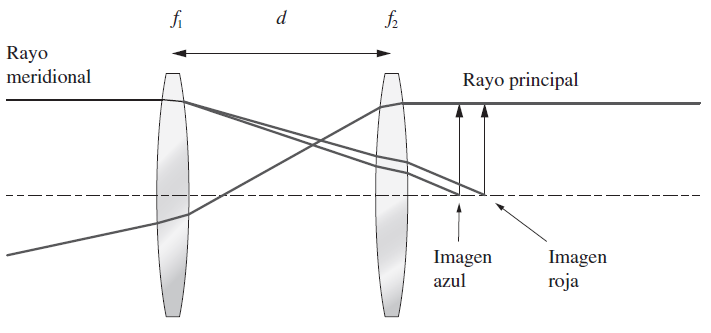
\includegraphics[scale=0.8]{Imagenes/Aberraciones_02.png}
    \caption{Corrección de la aberración cromática lateral en un sistema de dos lentes iguales, incluyendo el mismo tipo de vidrio.}
    \label{fig:figura_V_02}
\end{figure}
La distancia focal efectiva del sistema, usando la ecuación:
\begin{align*}
\dfrac{1}{f} = \dfrac{1}{f_{1}} + \dfrac{1}{f_{2}} - \dfrac{d}{f_{1} \ f_{2}}
\end{align*}
está dada por:
\begin{align}
\dfrac{1}{F} = (n - 1) \, K_{1} + (n - 1) \, K_{2} - d (n - 1)^{2} \, K_{1} \, K_{2}
\label{eq:ecuacion_V_15}
\end{align}
donde $d$ es la separación entre las lentes y $K_{1}$ y $K_{2}$ son unas constantes que dependen de los radios de curvatura de las caras de las lentes.

Ahora, si deseamos que $F$ sea constante al cambiar el valor de $n$ con el color, imponemos la condición:
\begin{align}
\dfrac{\dd{(1/F)}}{\dd{n}} = 0
\label{eq:ecuacion_V_16}
\end{align}
Por consiguiente, derivando la ecuación (\ref{eq:ecuacion_V_15}) con respecto a $n$:
\begin{align}
K_{1} + K_{2} - 2 \, d (n - 1) \, K_{1} \, K_{2} = 0
\label{eq:ecuacion_V_17}
\end{align}
Las distancias focaes de las lentes están dadas por la ecuación (\ref{eq:ecuacion_V_06}), por lo tanto encontramos que:
\begin{align}
d = \dfrac{f_{1} + f_{2}}{2}
\label{eq:ecuacion_V_18}
\end{align}
El sistema estará libre de aberración cromática lateral si la distancia entre las lentes es igual a la semisuma de sus distancias focales. Aunque este sistema no tiene aberración cromática lateral, llamada también de amplificación, tiene sin embargo una gran aberración cromática axial. Este resultado será muy útil al diseñar oculares para microscopios o telescopios, donde es mucho más deseable corregir la aberración cromática de amplificación que la axial, ya que esta última es muy pequeña debido a lo reducido de la pupila de salida.

Si en un sistema compuesto se acromatizan de manera individual cada una de las componentes, el sistema estará libre de aberración cromática de amplificación, independientemente de separaciones entre las componentes, además de estar libre de la aberración cromática axial.

\section{Aberración de esfericidad.}

La aberración de esfericidad es la más importante de las aberraciones de Seidel o monocromáticas, ya que es la única que afecta a todo el campo, incluyendo las cercanías del eje óptico. Su nombre viene del hecho de que esta aberración se produce aun en las superficies perfectamente esféricas, como se muestra en las figuras (\ref{fig:figura_V_03a}) y (\ref{fig:figura_V_03b}), para una superficie reflectora y una refractora. Note que la posición del foco depende de la altura del rayo sobre la superficie refractora.
\begin{figure}[H]
\begin{subfigure}{0.5\linewidth}
    \centering
    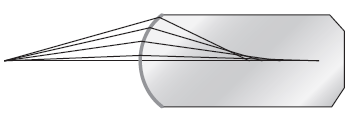
\includegraphics[scale=0.8]{Imagenes/Aberraciones_03a.png}
    \caption{Esfera refractora}
    \label{fig:figura_V_03a}
\end{subfigure}%
\begin{subfigure}{0.5\linewidth}
    \centering
    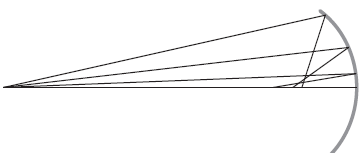
\includegraphics[scale=0.8]{Imagenes/Aberraciones_03b.png}
    \caption{Espejo esférico.}
    \label{fig:figura_V_03b}
\end{subfigure}
\caption{Aberración de esfericidad en una superficie esférica, a) refractora y b) reflectora.}
\end{figure}
La envolvente de los rayos refractados forma una curva característica llamada cáustica, la cual es muy fácil de observar en una taza de café iluminada por el Sol o un foco, como se ve en la figura (\ref{fig:figura_V_04}). 
\begin{figure}[H]
    \centering
    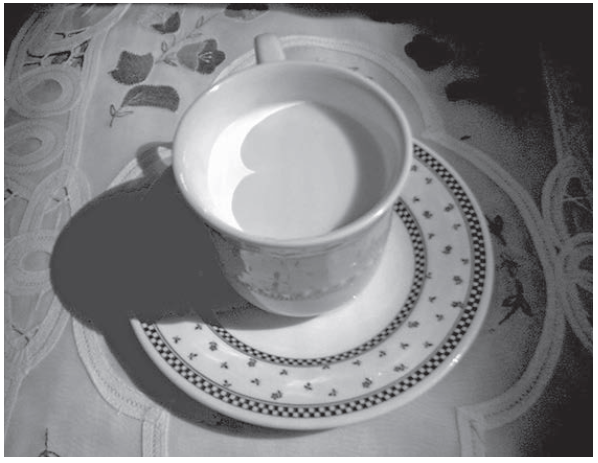
\includegraphics[scale=0.7]{Imagenes/Aberraciones_04.png}
    \caption{Cáustica que se observa en una taza de café.}
    \label{fig:figura_V_04}
\end{figure}

\subsection{Superficies esféricas refractoras libres de aberración de esfericidad.}

La aberración de esfericidad es una desviación de los rayos que produce diversos puntos de convergencia; éstos se pueden observar cuando el objeto es un punto luminoso colocado sobre el eje óptico, lo mismo que la imagen. Tanto una superficie simple como una lente tienen este tipo de aberración.

Al calcular la aberración de esfericidad se usa $l$ y $l^{\prime}$ para las distancias paraxiales, que corresponden a los rayos cercanos al eje óptico. Para los rayos alejados del eje se usa $L$ y $L^{\prime}$ a fin de utilizar las fórmulas generales de la refracción. Como todos los rayos parten de un solo punto, tenemos que $L = l$; pero no necesariamente $L^{\prime} = l^{\prime}$, debido precisamente a la presencia de la aberración de esfericidad.

Consideremos ahora la expresión exacta I.33 que se halla en el primer capítulo. Si sacamos fuera del paréntesis el término $(\sin I - \sin U)$, obtenemos: 




 



\end{document}